% This example An LaTeX document showing how to use the l3proj class to
% write your report. Use pdflatex and bibtex to process the file, creating 
% a PDF file as output (there is no need to use dvips when using pdflatex).
% Modified 

% This dissertation was built upon base template provided.

\documentclass{l3proj}

\begin{document}

\title{Team I: ResDiary Restaurant Recommendation System}

\author{Vladimir Bardarski \\
        Paulius Dilkas \\
        Domantas Jurkus \\
        Eduard Kalfov \\
        Josh O'Brien \\
		Joseph O'Hagan}

\date{31st March 2017}

\maketitle

% ##################################################
% LAST EDIT: 	06/03/17	Joseph
% ################# Comment Log ####################
% ##################################################
\begin{abstract}
The abstract shall go here! Here is some things to keep in mind while writing it.
\end{abstract}

\begin{itemize}
\item The abstract is likely the first substantive description of your work read by an examiner. View it as an opportunity to set accurate expectations.
\item The abstract is a summary of the whole thesis. It presents all the major elements of your work in a highly condensed form. (Write it having written the rest of the paper) The paper sets the abstract.
\item It must be capable of substituting for the whole paper when there is insufficient time and space for the full text.
\item Keep it short and snappy. 
\item The primary function of your thesis (and by extension your abstract) is not to tell readers what you did, it is to tell them what you discovered.
\item Approximately the last half of the abstract should be dedicated to summarizing and interpreting your results.
\item The most common error in abstracts is failure to present results.
\end{itemize}

% Comment out this line if you do not wish to give consent for your work to be distributed in electronic format.
% We hereby give consent - spread the knowledge - pending on result of project
\educationalconsent
\newpage

%==============================================================================

% ##################################################
% LAST EDIT: 	06/03/17	Josh
% ################# Comment Log ####################
% 	A. 	We mention the integration but the final 
%		state of the system is for it to be used
%		as a proof of concept / prototype by RD.		<--	Joseph 
% ##################################################
\section{Introduction}
\label{sec:intro}
% An introduction, explaining the purpose of the document, a very brief outline of the project and a summary of the structure of the rest of the document (approximately 1-2 pages).

The Professional Software Development (PSD3) course at The University of Glasgow requires students to engage with the practices and methodologies used in modern large-scale software engineering. The purpose of this dissertation is to document the development of the software project created as part of this course by Team I. 

% ---------- A ----------
The project was to build, over the course of several months, a recommendation engine for the Glasgow-based company ResDiary.
The main deliverable was a system capable of producing sensible restaurant recommendations for existing ResDiary users; a system that could be integrated into the existing ResDiary platform at a later date. 

Our team consisted of six third-year Computing Science students. Within the group there was a broad range of skills, interests and experience - with two members actively working as software professionals, and another having participated in an internship. For some members, however, this was a first opportunity to interact with a real client. 

In this document we outline, in detail, the entire process: from the initial requirements gathering with our customer, through to final system delivery. 

In section \ref{sec:background} we present the background to the project, the motivations of the customer and how we arrived at the agreed deliverables.

%this will surely be expanded to enumerate each separate section better I would like to discuss in detail the practices, issue-tracking, the team work/team load - Josh etc.

In subsequent sections \ref{sec:alice} through Section \ref{sec:reflections} we explore the challenges we faced through development and the steps we took to resolve them, explore the impact of team dynamics on the outcome and reflect on what we have learned from the experience. We also explain how we applied the good development practices learned in PSD3. In particular we highlight the role of version control, agile development and issue tracking.

\newpage

%==============================================================================

\section{Case Study Background}
\label{sec:background}
% A description of the case study background and context. This should include a description of the project customer (what was the nature of the organisation you were working for), their objectives for the project, and a summary of what was actually achieved. Where appropriate, this section should also make reference to similar related projects in order to make the context clear (approximately 4-5 pages).

\subsection{Customer}
\label{sec:customer}
% ##################################################
% LAST EDIT: 	18/03/17	Josh
% ################# Comment Log ####################
% ##################################################

% The customer organisation and background.

% Here we want answer the question of who are ResDiary and what do they do.
% Additionally answer who played the customer role of ResDiary to us on the project.

% Who are ResDiary?
ResDiary are a Glasgow-based online restaurant reservation service; a commercial organisation providing a comprehensive, easy to use booking and table management platform for use by the hospitality industry. The company provides 24-hour reservation services through both social media and their own booking portal ResDiary.com. Diners can browse restaurants, book tables and place reviews. Restaurants can access tools which let them optimize their yields, manage their reservations and attract new diners. Their global service sees 9.7 million bookings every month, and their platform is used by over 6,500 restaurants across 58 countries. 

ResDiary senior software engineers Adam Connelly and Ian Strachan acted as customer representatives throughout the duration of the development. They helped us understand the company line-of-thought behind the project, in addition to providing useful feedback, answering queries and supplying the team with the anonymised ResDiary booking data we required.


\subsection{Customer Objectives And Rationale}
\label{sec:custobjectives}
% ##################################################
% LAST EDIT: 	23/03/17    Joseph
% NOTE: 		Reference papers on Amazon / Netflix Models / Netflix Prize
% NOTE:         Added more specifics on Netflix Recommendations - make sure to tie in to our final output
%               Need to demonstrate that the research was RELEVANT
% ################# Comment Log ####################
%   Really explain why the project is beneficial to the customer - why would recommendations increase business, etc. - this was question / critique of project motives section of the presentation -- Joseph  
% ##################################################

% The rationale and initial objectives for the project.

% Initial Meeting and the customer's motivation for the project.

The initial customer meeting occurred on October 19th and was led by Ian Strachan. This was our first contact with the customer and served as the customer requirements elicitation meeting. The meeting began with an overview of the ResDairy business \ref{sec:customer}, a discussion of the services they provide and an explanation of their technology stack. The ResDiary daily operation involves gathering large quantities of valuable customer data. This collection of big data, however, is currently unused beyond supporting basic business needs (i.e. retrieving booking records). The developers view this as a significant shortcoming of their system.

As such, therefore, the company is exploring potential ways to exploit this vast quantity of valuable data. The developers had conducted some research into the area, and discovered that none of their competitors currently offer a restaurant recommendation service within their booking platform. Thus, if they were able to develop a system which would make recommendations to users based on their previous dining habits and similarity to other users, they would gain a competitive edge. It would also help increase restaurant discovery on their platform, which is beneficial to both restaurants and potential clientele. 

The inspiration for the idea stems from the similar system provided by online services such as Amazon and Netflix, which push recommended products and films respectively to their users. The Netflix model, in particular, was the closest reference point for the system they wished to develop. A parallel between making recommendations based on a user's film history and their similarity to other users, and a similar recommendation engine using ResDiary's dining history is easy to see. As a starting point for our own research, they suggested looking into the Netflix Prize - a competition held by Netflix starting in 2006 challenging participants to better their own recommendation algorithm. 

The goal of the algorithm was to accurately predict a user's rating of a film based solely on previous user ratings and no additional information about either the users or films. A set of training data (a subset of Netflix's real user data) with half a million user ratings was provided to participants, with the algorithm using this data to predict user ratings for a disjoint subset of the user data. No information other than user ID, film ID and date of rating was provided. Our Resdiary project followed a similar structure. ResDiary's users, as with Netflix's, leave review scores ranging from 1 to 5. We were given a subset of their user data which we split into further subsets for training and for evaluation. The research provided an excellent springboard from which to launch our own collaborative filtering model. With such a strong similarity between the requirements of our system and theirs, it was a natural choice.

We also spent time discussing what the customer viewed as the end state of the system - whether it would be integreated into the existing ResDiary portal or whether the output would suffice as a proof-of-concept prototype. They were initially undecided in this regard, partially due to an internal transition in their own development frameworks, and thus suggested our initial aim should be to focus on the creation of the recommendation engine. The decision regarding the final state of the project ultimately would not be made until midway through the development cycle when the customer decided to view the project as simply a proof-of-concept. Nonetheless, at all points during development, due consideration was given to the future integration of our system with ResDiary. 

\subsection{Project Scoping}
\label{sec:ourinitobjectives}
% ##################################################
% LAST EDIT:  18/03/17  Josh
% NOTE:         JOSH: Expanded on importance of requirements.
% NOTE:         References: importance of requirements gathering, cost of making corrections 
% ################# Comment Log ####################
% If required (page count) maybe cut down requirements engineering and incorporating customer 
% feedback in reflection point - we did it pretty well though so there wasn't much to improve
% ##################################################

The risks and costs associated with a project of this nature demand thorough background investigation and cogent planning before development proper commences. The cost of correcting errors grows enormously in the latter stages of a software project.

Our first major task was to formalise our discussions with the client and produce a requirements specification to serve as a project proposal document. The goal was to have a clear outline of the scope of the project and a set of deliverables to present to the client at the next meeting on November 16th. Our requirements gathering occurred in tandem with conducting the necessary initial background research on machine learning and recommendation systems. 

The proposal document included an array of requirements that the team agreed upon, based on our interpretation of the customer's initial project pitch. It was important that our requirements were reasonably comprehensive and realistic, but we accepted that they would be continually revised and refined as the project developed. 

\subsubsection{Initial functional requirements:}
\begin{itemize}
\item The recommendation engine must accurately suggest restaurants based on the users' dining history and similarity to other users with similar eating preferences.
\item Recommended restaurants should be in close proximity to where the user typically eats or the geographical location of where they are currently searching.
\item The recommendation engine may recommend restaurants that  the user has previously visited should the user allow this option.
\end{itemize}

\subsubsection{Initial nonfunctional requirements:}
\begin{itemize}
\item The engine should be written to allow for easy integration into the existing ResDiary system.
\item The system should give a response within one second after receiving the request (provided data is stored locally).
\item New users should be presented an optional quick questionnaire to gather initial data.
\item User and restaurant locations should be interpreted using coordinates rather than city name as those are of arbitrary precision within the dataset.
\end{itemize}

To help us understand the actual scenarios in which the system might be used, we prepared a set of user stories (ranked by priority). They provided a quick, intuitive way to ensure we had covered all the conceivable use cases the customer may require. We also prepared a high-level system UML diagram and a step-by-step work-flow of how the system would generate the actual recommendations. Due to the customer's ambiguity regarding the final state of the system, the endpoint was left intentionally vague to allow for flexibility. Instead the emphasis was to build and produce the most accurate recommendation for a given user. 


\subsection{Refinement of Requirements}
\label{sec:custrefineinitobj}
% ##################################################
% LAST EDIT:  15/03/17  Joseph
% NOTE:         Needs reworking
% NOTE:			Needs referencing
% ################# Comment Log ####################
% If required (page count) maybe cut down requirements engineering and incorporating customer feedback in reflection point
% ##################################################

% The suggested alternative was to use a nightly build system which the team would utilise in the final version of the system (!R! REFERENCE TO SPARK REFLECTION !R!).

At the November 16th meeting we presented and discussed our project proposal with the customer.

They felt we had a good understanding of their vision. They broadly agreed with the proposed requirements and could envision how our high level system would operate (and potentially integrate into their existing one). We briefly explained that there were two major models for building recommendation systems: collaborative-based filtering and content-based filtering. The high level system architecture accounts for this by allowing multiple 'recommenders' to each implement a different approach to producing recommendations. These recommendations are then combined and filtered for the final output. The customer expressed strong interest in the potential of "fine tuning" this system, through altering the significance placed on individual recommenders. 

There were, of course, areas of concern. Our proposed response rate of one second to respond to a request was queried. They felt that they needed to further clarify the volume of data the system would be expected to work with in a real world deployment. This may put a constraint on our ability to realise that performance. We discussed the alternative of using a nightly build system, as this how they expected the system would operate in a real world setting. In addition, they recommended developing a lightweight front-end application to display the recommendations. This would be a lightweight app, rather than any actual integration with their system, but they rationalised its throwaway nature by suggesting it would help them better understand our system, assist with demonstrating its functionality and most importantly provide a clear indication it was producing sensible results. 

We made modifications to the specification document to incorporate the customer feedback. In particular, the team felt the need to revise the non-functional requirements of the project. The disputed "one second local response rate" requirement was rescinded and in its place we inserted two new requirements:

\begin{itemize}
\item Provided the data is not stored locally, the system should be set up to allow for nightly updates to the recommendations.
\item Have the ability to “fine tune” the recommendation engine by altering the weighting significance of different components of the recommendation such as distance, price, 
reviews, etc.
\end{itemize}

Furthermore, a soft goal developed within the team to produce a more comprehensive front end application to showcase the recommendation system. While some members felt this justified being included and defined formally within the specification document, the majority instead felt the focus of the project should be on creating the most accurate recommendations. We elected to delay defining an exact end state until the customer clarified exactly what they required. We agreed, eventually, that should clarify not be forthcoming, we would press for clarity on the issue during the scheduled January 26th meeting, and define an agreed handover state for the project. 

While some of the team felt this justified being defined within the specification the majority instead felt the focus of the project should be on creating the most accurate recommendations and delay defining an end state until it was defined by the customer. Should the customer not provide clarity earlier it was decided to press for clarity on this issue during the scheduled January 26th meeting and define a agreed handover state for the project. 

Thus, prior to this meeting, development efforts were split between the creation of a prototype system (which implemented a basic content-based filtering model) and on the long-term solution (with multiple recommenders) to the project. The prototype system was demonstrated during an interim meeting on December 7th, where the technical decisions of the long term solution were discussed at length. Following this meeting, implementation of the system proper commenced. 


% \subsection{Technical Research \& Prototyping}
% \label{sec:techresearchproto}
% ##################################################
% LAST EDIT:  15/03/17  Joseph
% NOTE:         Perhaps best to merge with above subsection
% ################# Comment Log ####################
% ##################################################

\newpage
\subsection{Defining the End Product}
\label{sec:jandefinedstate}
% ##################################################
% LAST EDIT:  15/03/17  Joseph
% NOTE:         Needs reworking
% NOTE:			Needs referencing
% ################# Comment Log ####################
% ##################################################

As we discuss in the previous sections, the decision to define an exact final handover state for the system was deferred until the end of the third development sprint. During our January 26th progress meeting, the team pressed the customer for clarity on how they envisioned the end product. 

It became clear that the customer wished to view the project as a "proof-of-concept" demonstration, with their intended use being to assess the worth of creating a similar system for use with their existing portal. Additionally, they wished to learn from our work, as both developers had little experience in the field of machine learning. The business use of our system would be as a prototype to justify the development resources required to develop their own solution.

With the final handover state of the system now clarified, the team decided that a redesign of the front end of the application was necessary. We noted while giving a demonstration of the software to a non-technical member of the ResDiary team, that the system was not properly communicating the recommendations being made. It was unclear to a non-technical user how the system operated and whether or not the results it produced were sensible. Given it was confirmed that the primary audience of our software will likely be non-technical users (being given a demonstration), there was urgency to produce a more intuitive, friendly front end. 

The following requirements were discovered and added to the project, with the aim of producing a front end redesign which visually demonstrated that the system was producing accurate predictions:

Functional
\begin{itemize}
\item The front end display should display recommendations for a random pool of users to simulate typical use of the system.
\end{itemize}

Nonfunctional
\begin{itemize}
\item The front end be designed such that it is aesthetically clear that the recommendations made are sensible and accurate.
\end{itemize}

%Ensure a reference is provided to feature removal
We also elected in the aftermath of the meeting to drop the proposed nonfunctional requirements of implementing recommendations for new users. A more detailed account into and justification of this decision can be found in Section 3.

\subsection{Delivered Software}
\label{sec:finsoftware}
% ##################################################
% LAST EDIT: 	06/03/17	Joseph
% ################# Comment Log ####################
% ##################################################

% Information on the final software that was delivered to the customer.
In Section \ref{sec:ourinitobjectives} we discuss the specifics of Netflix Recommendations and the Netflix Prize competition so we need to make sure to tie this, the influence and similarity between that system and our final output. 

Additionally we need to demonstrate that the research conducted was RELEVANT.

This section can only be written after the software is in its final handover state.
\newpage


%==============================================================================
\section{Alice}
\label{sec:alice}

This is a example of how to include an image from the figures directory.

\begin{figure}
\begin{center}
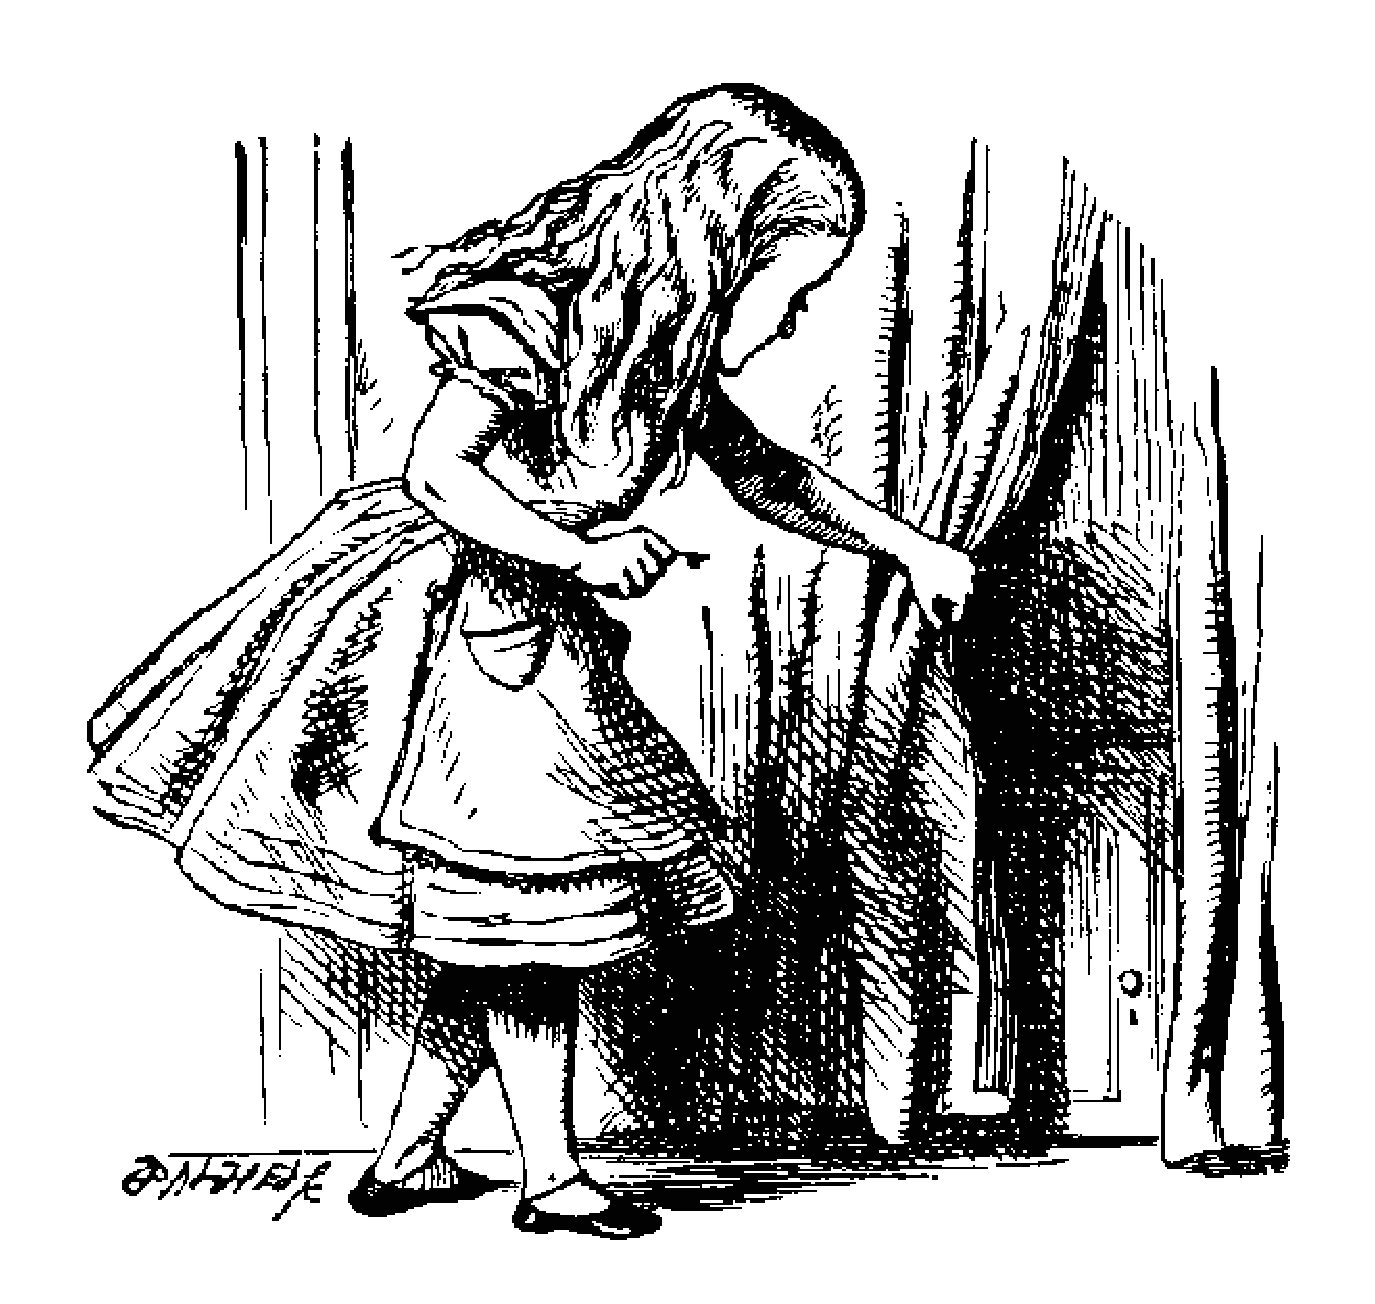
\includegraphics[width=7cm]{figures/alice}
\end{center}
\caption{Behind it was a little door}
\label{fig:alice}
\end{figure}

This is an example of how to reference an inlcuded figure (see Figure \ref{fig:alice}).


%==============================================================================
\section{Reflections}
\label{sec:reflections}
% ##################################################
% LAST EDIT: 	14/03/17	Joseph
% NOTE:	Currently misc. thoughts / notes
% ################# Comment Log ####################
% ##################################################

% Several sections that reflect on your experiences during the team project. Each section should discuss one theme, characterised by incidents or events that occurred during the team course of the project from which you learned (approximately 12-15 pages).

% STRUCTURE PLAN ??? -> Unless you propose something better

% Currently I see the layout of Section 3 as follows:

% Section on technical choices containing the major decisions - Models / Python / Spark - tie in requirements engineering (closely associated with technical decisions) and testing as a technical reflection (this leaves remaining reflection points Agile, non-technical and process focused)

% Section on Scrum methods and general practices which could have been done better

% End with discussion on whether Scrum was correct method to use or if it would have worked better if followed more strictly - leads into conclusion as I expect it will feature a discussion of this point 



\subsection{REFLECTION POINT - Technical Overview Section}
\label{sec:techoverviewreflection}
% ##################################################
% LAST EDIT:  18/03/17  Joseph
% NOTE:         Temp notes / thoughts
% ################# Comment Log ####################
% Development Langauges, Models and Spark being 3 sub-sub-categories within this encompassing category.

% Reference general importance of design decisions here
% Reference specific sub-sub-category when applicable

% If we tie in testing and requirements engineering here the remaining reflections are less technical and
% more agile reflections
% ##################################################

% This section should be a mainly postive reflection of the technical choices of the project.

% The occasional limitation can be mentioned in the passing such as the use of Python scaring the customer off integration (theory) 
% and the drawbacks of the collab not allowing for training based on only new data (this if anything is a requirements engineering failure
% that could have been picked up earlier but customer did not consider until after seeing operation of prototype and use of data in its creation)
% Spark was fine. I have no gripes about using Spark.

1. Talk about why the technical choices are significant development points in the software development process.
2. Talk about how preemptive commitment too early is bad and should be avoided - reference case study - saying team used this as an warning. Use this as reference throw over to requirements engineering reflection point. 
3. Introduce the three major technical decisions of our project
4. Tie in testing and use as a reference throw over

Preemptive commitment to particular design choices too early in the software development cycle leaves a software project at high risk of failure (reference a case study where an incorrect design decision lead to failure - lecture 1 / 3 recommended reading?). Summary of how this system failed in relation to incorrect design choice. 

Aay the team used this as a warning for the major design decisions - Development language, Models, Spark - that were involved with our project which are detailed below.

State how the technical choices do not occur in isolation rather they are heavily work with the requirements gathering stage (reference lead in)

Additionally discuss how they are related to the testing of the system (reference lead in) 

However the technical choices of a software project are not made in isolation rather they are heavily influenced by the requirements engineering process of the 

\begin{itemize}
\item Demonstrate that the research conducted was relevant
\end{itemize}


\subsection{REFLECTION POINT - Python}
\label{sec:pyreflection}
% ##################################################
% LAST EDIT:  15/03/17  Joseph
% NOTE:         Temp notes / thoughts
% ################# Comment Log ####################
% ##################################################

Misc Points:
\begin{itemize}
\item What alternatives did we consider - C Sharp / Scala
\item What were the benefits of using it - already familiar / libraries / industry standard
\item The choice of Python is mentioned in a retrospective as the choice was slow and not well discussed and we just jumped into it - how did we ensure this did not occur with other major technical decisions
\item Did Python influence other later choices - Spark, etc.
\item What were the limitations of using Python
\item Was using Python the correct choice in the long term 
\item Reference papers and libarires to justify why Python 
\item Demonstrate that the research conducted was relevant
\item Was Python the correct choice - research conducted proved Python and C\# integration wouldn't be an issue. However as the customer lacked Python knowledge it probably deterred them from wishing to integrate our system into their existing one. Had the system been created in C\# then perhaps this would have been different. Perhaps this should have been better discussed with the customer in the initial stages of the project.
\end{itemize}


\subsection{REFLECTION POINT - Models}
\label{sec:modelreflection}
% ##################################################
% LAST EDIT:  15/03/17  Joseph
% NOTE:         Temp notes / thoughts
% ################# Comment Log ####################
% ##################################################

Misc Points:
\begin{itemize}
\item Explain how the collaborative filter works and WHY it is applicable for our needs
\item Explain how the content based filter works and WHY it is applicable for our needs
\item Reference papers and other models (Netflix) to justify choice
\item What were the limits of the models - customer asked to only retrain on new data but limit of model disallows this - need for specific type of data that is not always present within the data set.
\item Did we choose the right models
\item Did the models impact later decisions
\item Probably suggest some alternative models which could have been explored
\item Demonstrate that the research conducted was relevant
\item Tie in the Netflix competetion and Netflix model as referenced in \ref{sec:initcustobjectives}
\item Knowing the complaints of lacking various fields, columns, data was the model choice actually correct? From the outset it was the more obvious choice but would an alternative have yielded better results working with the data sets we were being given?
\item Jeremy asked about the reusability of our system and the models during the presentation - mention ours is tailored to our specific system and results to improve the accuracy of the results and predictions
\end{itemize}


\subsection{REFLECTION POINT - Apache Spark}
\label{sec:sparkreflection}
% ##################################################
% LAST EDIT:  15/03/17  Joseph
% NOTE:         Temp notes / thoughts
% ################# Comment Log ####################
% Readded after accidental deletion
% ##################################################

\begin{itemize}
\item Team decided the entire team should spend time over Christmas playing around with Apache Spark to ensure common understanding of the system between team members. This may not have been the best use of resource and instead team could have split earlier and the front end developers not bothered playing around with it as they did not end up touching it directly during the development of the project. 
\item Common knowledge was gained though but a more typical front end, back end split in focus may have been beneficial and resulted in an improved front end application sooner.
\item Why was the decision made to use Spark?
\item Did any previous decisions (models / languages / tools) influence our choice of Spark
\item What were the alternatives to using Spark
\item What were the benefits of using it?
\item What were the limitations of using it?
\item Was Spark the right choice?
\item What impact did deciding to use Spark have on the project?
\item Demonstrate that the research conducted was relevant
\item Spark seemed fine for our purposes.
\item Future proposal for system / talk about scalability and benefits of using Spark
\item Quote the numbers Mason! The numbers! (You know the ones Eduard likes to mention)
\end{itemize}


\subsection{REFLECTION POINT - Requirements Engineering}
\label{sec:teamstructure}
% ##################################################
% LAST EDIT:  20/03/17  Joseph
% NOTE:         Temp notes / thoughts
% ################# Comment Log ####################
% - References the cost estimation reflection point as an improvement - tie those two together
% - References scenarios which flows to testing via test scenarios / acceptance testing - ties those two together
% Reference back in subsequent reflection points to reduce lead in repetition 
% ##################################################

% Perhaps tie in the requirements risks and perhaps suggest methods of dealing with such risks via papers

% Basically we've reflected on the technical choices now why was it important that the requirements were engineering properly to better inform the technical choices and what could have been done to do this process even better

From the outset of the project the team were aware of the need to properly capture the requirements of the project. It is widely documented that two of the primary reasons for software failure is due to building the wrong system and building the system incorrectly (said in lecture 3 - get academic proof) both of which were major threats to the development of our project. The team was mindful of how easily building an incorrect system, one not based off similarity between users, or selection of the incorrect machine learning model and subsequent project failure could occur in our project. 

Adhering to the advice of avoiding early commitment to a particular design solutions during the requirements elicitation process as is discussed in Section (reference case study reflection at technical overview point) the team left the decision regarding the specific models and tool choice until after this phase was conducted. Although the requirements would evolve as the project developed, as is to be expected, the team felt with the correct initial system goals established the team could easily justify decision designs in relation to the key goals of the system. Such technical decisions, specifically the choice of development language, machine learning models and clustered computing framework, are discussed in Sections (reference all three technical reflections) respectively. 

Knowing the significance of the requirements engineering process for the sucessful development of the project, the team dedicated the first milestone to ensuring the proposed system to be built was correct. This occurred in parallel with technical research into similar systems and their creation (reference Netflix research from section 2). To ensure the team captured all functionality of the system the team, having conducted the initial customer interview, prepared a requirements specification document which was later refined through customer discussions (reference section 2 requirements section). 

Within this document the team elected to use the user stories method of requirements specification in order to create an all encompassing set of stories which reflected the proposed features and functionality of the system. As the recommendations are made to ResDiary customers the team felt user stories provided a good a boundary artifact between the proposed users, customers and developers (taken from PSD lecture 15 key point) and that user stories were a natural choice opposed to alternative specification techniques such as use case diagrams because… 
% Try to sell the idea that user stories are the natural choice for our project as user stories are written from the customer perspective and the recommendations are being made to the end customers

Although some modifications were necessary, as is to be expected, the team found that proposed the user stories modelled the customer requirements with a good level of accuracy (reference section 2 refinements after initial meeting). In addition to this the additional proposed features, generating recommendations for new users and the ability to recommend previously visted restraunts, that the team suggested were recieved with good feedback by the customer. They believed such features tackled aspects of the problem they themselves had not yet considered and felt we had a good understanding of the system. 

% Establish that task estimation was not properly conducted then reference away to specific reflection into that topic
One shortcoming of the use of stories however was the measure of priority attached to each user stories and the subsequent task breakdown by association. The team did not conduct a formal task estimation procedure beyond the breakdown of the user stories into smaller, more general tasks. This was in part due to the lack of technical knowledge into the subject area from the team at this stage in development though the team should have conducted proper task estimation to assist with project planning and management as is discussed here (reference planning and cost estimation reflection point). 

% Transision into this better and potentially expand on
Another area of improvement in the requirement gathering process would have been the inclusion of use scenarios in the “Given, When, Then” format. This is a natural progression of user stories as it expands upon an individual story to provide an example of it in action. Such scenarios could then be utilised to allow for further refinement discussions to occur with the customer in order to establish conditions of system acceptance and thus form the basis of acceptance and scenario testing to be conducted on our system. Such tests are absent and would have improved our testing process as is discussed in Section (reference testing reflection point).  

% Tidy up the ending better - more postive - team did well in this regard and so should end on positive note
Although the aforementioned could have utilised to improve the team's cost estimation and test process for the project, the team established a good understanding of the customer's vision and corresponding system requirements. This ultimately showed during the various customer demonstration where by second to last meeting they encouraged to the team to follow where we saw the development of the system going as they were already impressed and pleased with the results. This level of confidence placed in the team we feel showed we had a good initial grasp of the system and thus were able to deliver and take steer the project in the direction we saw it heading towards the later stages of the project. 

% Here downwards is notes
\begin{itemize}
\item (Lecture 13) Requirements gathering is an ongoing iterative process that runs concurrently alongside requirements analysis and capture - our project saw this in real effect due to the changing nature of the requirements of our project.
\item (Lecture 14) Requirements engineering is an iterative process of elicitation, capture and validation - talk about how we did this to ensure we were gathering the correct requirements.
\item (Lecture 3) Causes of software project failing - building system for wrong reason, building the wrong system, building the system wrong. We could tie in the dropped new user recommendation to a proposed goal which was later determined to be a requirement which would be built for the wrong reason. As such the feature was dropped to avoid building an incorrect system.
\item (Lecture 13) Cultural differences between engineers and customers - although the developers were technical they don’t know anything regarding machine learning or the development of a system such as ours - Requirements Risk
\item (Lecture 13) Vague requirements specification of end state of system / customer uncertainty regarding the final state of the system - Requirements Risk
\item (Lecture 13) A means of investigating poorly understood requirements (prototyping) - Managing Requirements Risk - perhaps we could have prototyped both a front end display and an integration method / discussed this with the customer earlier. This would have defined a determined end state of the system prior to January which would have allowed for an earlier split in development focus and resulted in either integration or improved front end. Granted one must also consider that technical decisions were still ongoing at this time.
\item (Lecture 13) Requirements evolution - occurred when we discovered potential features which were ultimately dropped (new user recommendations)
\item (Lecture 14) Avoid early commitments to particular design solutions during requirements elicitation
\end{itemize}


\subsection{REFLECTION POINT - Testing}
\label{testing}
% ##################################################
% LAST EDIT:  19/03/17  Joseph
% NOTE:       TODO
% ################# Comment Log ####################
% ##################################################

% Was a testing model used?
% Should a testing model have been used?
% Why was testing important for this project?
% When did the testing process start in the development cycle? 
% Was it easy/hard to test and why?
% Discuss why continuous integration was particularly important for the project
% Would a TDD test strategy have been suitable?
% Would the XP test strategy have been suitable?
% Are there test strategies specifically for machine learning projects which could have been followed
% Could we have used test scenarios with and determined the levels of outcomes are acceptable for each scenario
% Could we have set objective acceptance criteria and established the amount of error you and your users are willing to accept
% What statistical level of confidence do we have regarding the accuracy of the system in relation to our conducted testing

% Should our testing have better utilised statisical measures in relation to the system accuracy

% Could the testing have provided internal feedback on the efforts of the application. First, evaluate the application according to the acceptance criteria. Second, be prepared to support those assertions in statistical terms; for example, be 95 percent confident that the application will produce an answer within a given range. Last, have a high-level understanding of the underpinnings of the application, so that any deficiencies might be able to be ascribed to a particular application component.


% TODO: READ THE FOLLOWING AND NOTE ANY IDEAS
% http://pages.cs.wisc.edu/~dpage/cs760/evaluating.pdf
% 

Talk about why testing was significant for this project.

A suite of unit tests was written to ensure that each commit did not break the execution of the project.

\begin{itemize}
\item (Lecture 10) Continuous integration practices minimise the disruption caused by rapid, concurrent changes to software systems - explain why this was suitable for our purposes, concurrent development of aspects of the system (evaluator and recommender), etc - Testing / Code Reviews
\item Overlap between testing and evaluation.
\item Although there were considerations on testing the front-end portion of the project, it was agreed that such tests were not essential for the presentation of the recommendations.
\item Integration testing: The System recommender was tested in conjunction with other recommenders for integration.
\item Regression testing: A regression test for hyperparameter learning was written.
\item Mutation tests were considered but not used.
\end{itemize}

The unit tests were set up to run on Jenkins, a continuous integration environment.
Jenkins was set up to push notifications to the team's communication channel whenever a test case would fail. This enabled early notification of issues, allowing the team to patch up bugs early on.
Jenkins also provided coverage reports for the source files, indicating the percentage of classes, conditionals and lines covered.

What could have been improved:
A notable shortcoming was that tests were not written under any particular testing strategy. This lead to the discovery of several modules missing tests cases, and some tests using untested modules. Following a stricter test plan would have led to more systematic test development, allowing to uncover the beforementioned problems earlier.


\subsection{REFLECTION POINT - Scrum Lead In}
\label{sec:teamstructure}
% ##################################################
% LAST EDIT:  21/03/17  Joseph
% NOTE:         Temp notes / thoughts
% ################# Comment Log ####################
% Ending is real clunky but I like the idea of a lead in general reflection via references to the Scrum
% ##################################################


% !!!!!!!!!!!!!!! IMPORTANT NOTE TO SELF !!!!!!!!!!!!!!!!!!!!!!!!!!!!!!!!!!!!!!!!!!
%
% Scrum reflection story
%
% The way I envision the general reflection for the Scrum method being 
% examine each of our shortcomings in terms of team workflow (task backlog, communication, etc)
% and to possibly suggest Scrum / XP methods / extensions which could have been employed
% to avoid such failures from the team. This can then be used in the final reflection
% point comparing which framework we should have followed more closely. For example 
% following Scrum more closely with daily (very frequent) stand up meetings would have
% avoided the issue of lack of communication of what you are actively working on.
% Additionally Scrum task and priortiy reviews would have handled that issue, etc.
%
% !!!!!!!!!!!!!!!!!!!!!!!!!!!!!!!!!!!!!!!!!!!!!!!!!!!!!!!!!!!!!!!!!!!!!!!!!!!!!!!!!


% Now see this as a general lead in saying we used Scrum, highlight the overall performance and tease the key failures of our use of Scrum. Finish with a tie in to the final reflection point on whether Scrum was the correct practice to use for the project. 

Lead in with a general why Agile is used for large projects such as ours.

As is often a common practice in industry (get a reference backing up claim) the team did not adhere strictly to one specfic agile framework. Instead the Scrum methodology was used as the overarching framework with additional agile practices from alternative methods, such as prototyping and extreme programming, being adopted as the team felt their use necessary and applicable. While this behaviour ensuresd a flexibile production envirnoment and the team found modertate success with the loose methodology it was not without its issues. Primarily this was due to the lack of discipline within the team to hold all of the key Scrum methods, as weekly stand up style meetings were cancelled in favour of a more open source style of development environment, and roles, as the team employed no product owner role and the scrum master was additionally on the development team. 

Ultimately this would come at a cost of the teams ability to collaborate effectively on the project as the lack of stand ups led to communication issues as is discussed in Section (reference communication issue). Additionally the lack of product owner and focused scrum master roles played into some disfunctionality within the team organisation structure as highlighted in Section (reference team structure). By not conducting incomplete work and priority reviews at the each sprint's end the team inevitably saw proposed features be dropped as is discussed in Section (reference dropping features) and examined more thoroughly in Section (reference backlog management). This however may also be a consequence of the lack of formal cost estimation procedures conducted during the project as examined in Section (reference cost estimation) and not the teams approach to the Scrum methodology. Finally the issue of if whether such failures could have been avoided through use of a different agile framework, the Extreme Programming framework, is considered in comparision to following the Scrum methodology more strictly and closely than was conducted by the team in Section (reference stricter Scrum vs XP - final reflection point).


\subsection{FINAL REFLECTION POINT - Scrum vs XP - Was Scrum The Right Choice}
\label{sec:scrumvsxp}
% ##################################################
% LAST EDIT:  15/03/17  Joseph
% NOTE:         Temp notes / thoughts
% ################# Comment Log ####################
% ##################################################

Comparision I see here being made now is should we have stuck with Scrum but follow the practice more closely with stand ups, product owner and scrum master - ensure to explain academic nature of project affecting that one in some regard, extensions to Scrum methods which could have been used to tackle specific problems, etc.

Contrast this against using the XP system for example.

Misc points:
\begin{itemize}
\item Our prototyping was beneficial - gave good understanding of working with the data sets in addition to seeing how and what the front end application would need to convey to non-technical people and people not familiar with the nature of the project. Spin here is to implement more forms of prototyping as this was beneficial and perhaps should have been conducted more. Not Scrum or XP but another framework that could have been adapted in. 
\item Time between meetings served as a good sprint dates - working on smaller iterations may have ensured better communication within the team.
\item Development typically did not change much within a sprint - XP difference here may not have made much of a difference though the dropped feature could have been explored earlier in the development cycle than the 2nd semester.
\item Task priority was a bit of an issue as we didn’t really do proper task estimation - XP would have solved that issue as it forces strict policy and task estimation.
\item Scrum has no engineering practices whereas our project definitely should have. XP would have forced pair programming from the start (rather than sporadic occurrences within sprints), ensured better, more thorough testing from an earlier stage in the project and avoided the whole code review “you deleted all my code you bastard” arguments.
\item User stories are originally from XP 
\item Scenarios are from XP - discussed in requirements engineering reflection point 
\item Instead perhaps it would have been better to adopt additional Scrum extensions of backlog refinement and burn down charts in addition to having more defined roles and stand up meetings.
\item Reference throughout to relevant subsection reflection points tackling each specific issue.
\item Although the team did not conform to the Scrum practice of holding daily, or frequent, stand up meetings and the consequences of this practice are discussed at length in Section (reference lack of stand ups / poor communication).
\item Look into Scrumban and Agilo for Trac - did a light version informally but it would may have improved the process to got all out and use this.
\end{itemize}


\subsection{REFLECTION POINT - Team Structure}
\label{sec:teamstructure}
% ##################################################
% LAST EDIT:  19/03/17  Joseph
% NOTE:         Temp notes / thoughts
% ################# Comment Log ####################
% REFERENCE: Developer Anarchy - article || paper on it
% REFERENCE: Sports model of team structure - roles
% ##################################################

% Mention Scrum master hybird role in this section
% Mention lack of product manager in this section
% Reflect on if a more focused scrum master would have improved the process
% Reflect on if a product owner would have improved the process

% Reflect on the transision from Anarchy to a sports model and how it improved the development efficency - improved communication / workflow / etc.

Initially the team elected to use an 'developer anarchy' team structure whereby any team member was free to work on whichever aspect of the system they were currently interested in working on. Despite being an unconventionally structure the team felt confident in our ability to effectively communicate and organise development resources. Anarchy also looked promising due all of the team feeling comfortable to work on both the back and front end functionality of the application as needed. Finally as the proposed system design allowed for concurrent development on different back end recommenders to occur the team believed that the anarchy development style was suited to the project.

During the December 8th retrospective which saw the closure of the first true development milestone, the team was optimistic about the team structure and felt a natural order had fallen into place. The team felt, however, that the organisation and communication could be improved as open communication regarding what developers where actively working on and opinions shared on completed work was absent. (This should have been a sign for code reviews). In addition it was highlighted that task allocation did not actively reflect what developers were actively working on and the team felt this too was adversely affecting the development efforts. Although measures were taken to refectify such behaviors, as is discussed in Section (LINK COMMUNICATION / TASK BACKLOG REFELCTION), at the next retrospective on January 26th it was highlighted that the same issues had occurred once more. Furthermore some team members began to feel underutilised and it was noted that components of the system, the front end, testing and content based recommender, had not seen as much attention as required. To combat this the decision was made to adopt the sports model of role based development structure as the team split into two separate development subteams (reference sports + role model). 

% After change to role system reflect on improvement to development (positive reflections)

The decision was made to focus testing on the back end.
There was a clear front end and back end team.
Back end employed naturally developed roles - content based, collaborative, system, evaluator, testing  

Why did it fail?
People did not communicate effectively
People did not wish to do what they viewed as less important tasks - front end / testing
Underestimated the complexity of building such a system and the time required to do so - prototyping, etc.
Mythical Man Month text - too many cooks in the kitchen for the back end development. Instead better to have one developer focus on the collab recommender, one focus on the content recommender, one focus on the evaluator, one focus on the system (NEO) recommender, one focus..., etc.

Anarchy would explain the lack of time estimates and product owner however.

Reasons for the failure of the anarchy include the following reasons:

\begin{itemize}
\item Failure to communicate between the team - people weren’t discussing what they were actively working on, tickets didn’t reflect what people were working on, people didn’t yield results in an efficient enough manner.
\item Failure to fully understand domain - anarchy structures require huge expertise of the problem domain which regardless of how smart you are you cannot gain a grasp of in a few weeks. There’s a reason we pay for years worth of experience in a field / industry.
\item Motivation took a hit over Christmas (it was the holidays)
\item Lack of trust between team as this was the first time we worked together as a team on a long term project.
\item (Lecture 6) The sports model of role based development structure - the team adopted this model in the second half of development.
\item (Lecture 6) Are any of the other models such as Laissez-faire suitable?
\item (Lecture 6 / Lecture 7) The team paid measure to the Mythical Man Month text in order to avoid too many cooks entering the back end development after the team split to focus on the front and back end split.
\end{itemize}

Changing to a more structured development system did have an effect on productivity (testing improved - we actually had some, front end redesign was rad, more defined roles resulted in better communication within the team)


\subsection{REFLECTION POINT - Code Reviews \& Branching \& Pair Programming}
\label{sec:codereviewbranch}
% ##################################################
% LAST EDIT:  19/03/17  Joseph
% NOTE:         Temp notes / thoughts
% ################# Comment Log ####################
% Very, very, rough
% Struggling to explain why it appeared that commits were fine which were in fact broken
% REFERENCE: Good Agile code commit practices
% ##################################################

% Code reviews - negative reflection (we should have done code reviews)
% Branching - neutral reflection (tutor guy didn't seem to like that we were all commiting to master so maybe talk cons of doing that in relation to lack of code reviews resulting in tensions with deleted code)
% Pair programming - positive reflection (that should have been done more often)

Story to paint here is the following:
\begin{itemize}
\item Start by explaining why the lack of branching
\item Explain why code reviews were needed
\item Explain how and why code reviews would have been beneficial - allow for branching and have code reviews upon merging / semi regularly
\item Suggest pair programming as an alternative to code reviews
\item Summarise the pair programming which occurred and why it was beneficial ending with it should have been done more
\end{itemize}

Explain why the system design was created to minimise unnecessary branching as some of the team felt that branching would encouraged delayed commits due to the additional costs of handling merge conflicts.

As the development of the system progressed and the system complexity increased it was highlighted minorly during the third and significantly during the fourth retrospective was that integration of new code was becoming an issue. Specifically that new code was being added to a particular recommender which would break the system evaluator component in addition to code was often being commit which was unfinished and being refined. Obviously such behaviour is not good Agile practice (reference good Agile practice article) though a potential explanation for this behaviour was due to lack of test strategy in place (reference test reflection point) which would result in the newly added code appearing to function correctly within the existing system, by passing all of the integration tests, whereas in reality it had in fact broken another component of the system. This was due to the integration tests correctly checking the code would generate the recommendations but not that the code was functioning correctly with the evaluation system.

Unfortunately as a result of poor communication between developers (reference communication reflection) this would often lead to another developer's work being deleted in order to fix the broken build which would lead to conflicts within the team. Obviously such behaviour is not acceptable within a development team as was highlighted during the fourth retrospective meeting. To combat this behaviour it was agreed to not delete another developers code without discussing it and justifying it to the developer who wrote the code. Furthermore it was agreed to stop submitting non-functioning code which was still a work in progress. The suggested methods were suggested due to time restrictions placed on the team as the work entered the final development sprint and the proposed solutions did work in the short term. However such practices are neither proper nor are they long term solutions. 

Instead the most obvious combat to this problem would be to conduct regular code reviews...

Misc Points:
\begin{itemize}
\item The system was designed such that branching was unnecessary for the project. Branching was somewhat discouraged throughout the project in order to reduce merge costs / time. Whether the time saved outweighs the time spent fixing and altering other people’s code remains to be seen.
\item Lack of code reviews meant that the code often had inconsistent styling.
\item Lack of code reviews meant a significant portion of time was spent fixing or altering other people's code to work with parts of the system they did not realise they had broken.
\item Lack of code reviews meant code which was WIP was deleted prior to it being fully implemented into the system - again lack of branching issue somewhat.
\item Suggested at the first retrospective but ended up avoiding. Would have reduced a number of problems with development cycle but you can't be perfect.
\item Highlighted in retrospective 3 with the code integration being highlighted.
\item Highlighted even more in retrospective 4 with code integration really being highlighted.
\item Reference potential methods or strategies for code reviews which could have integrated into the development.
\item Reference how other and often professional developers recommend doing code reviews.
\item Mention that pair programming was conducted and the benefits of doing it. Mention it should have been conducted more frequently, reference that it was beneficial when suggesting if XP was potentially better than Scrum.
\item Code reviews might have improved development efficency as less time spent refactoring and fixing broken code. Reduced arguments caused due to deleting other people's code prior to full implementation. Branching also would have fixed this as only get back to master upon passing all tests. This would require testing to have been more efficent as well thus suggesting test strategy should have been utilised to improve test efficency.
\item (Lecture 26) Outline of inspection methods - should probably mention which we should have used in the code reviews.
\item (Lecture 8) Change management and the conflicts caused from developers working in parallel and contributions are made to the master branch which are not fully implemented or break some aspect of the system. In hindsight this probably should have justified a separate branch which would be integrated into the master upon passing all of the tests with a successful build in Jenkins the continuous integration system.
\item Pair programming done for design / initial coding of front end of application. Similarly done for aspects of the back end development of the project - well somewhat pair programming where one guy would bounce ideas and assist another in the structure and functionality of that particular aspect of the project. Potential spin for the front end is that a more experienced front end developer Josh worked with a less expereienced developer Joseph and the benefits of this (see note on pair programming on wiki somewhere for similar argument)
\end{itemize}


\subsection{REFLECTION POINT - Dropping Features}
\label{sec:droppingreflection}
% ##################################################
% LAST EDIT:  15/03/17  Joseph
% NOTE:         Temp notes / thoughts
% ################# Comment Log ####################
% Currently a pool of notes
% Two types of feature dropping:
%  1. Dropped due to straying from cutomer vision - new user recommendations
%  2. Dropped due to lack of time / project management / planning - recommendation reasons / system recommender saying contribution states from various other recommenders on the system recommendation / comparision of our system against other methods such as random guessing, etc - mention then fire off to relevant reflection point section 
% ##################################################

For example, if you found that you had to drop a feature during an iteration, discuss the reasons why the feature had to be dropped. Had you given yourselves too much work? Was the feature harder to implement than you realised? Had you got your priorities wrong? Then consider looking at the literature (see the recommended reading for PSD3) on project planning and estimation. Was your experience typical of a software project? What steps do other developers advocate for improving estimation?

% General lead in regarding that feature dropping occurs for many reasons

The dropping of proposed features from the development schedule can transpire in a software project for a variety of reasons yet they still provide an excellent insight into the ongoings of the development cycle. It may be that the proposed feature was identified as an example of scope creep which would overcomplicated the system design and stray from the customer's original intent from the system. An example of this can be seen within our project where the team initially proposed to implement recommendations for new users in addition to making recommendations for existing users. This feature was later dropped after conducting some initial research into the subject which found the problem was a searched based recommendation opposed to the similarity based recommendation which was the customer's intended desire. In this occurrence the team made the correct decision to halt the development during the research phase thus limiting the cost to the development costs to the project. 

Why does scope creep occur?
1. Poor Requirements Analysis
2. Not Involving Users Early Enough
3. Underestimating the Complexity of the Project
4. Gold Plating

Discuss which of these made their way into our project and methods of avoiding them. End with the team did well to kill the feature in the crib at the RnD stage.

Potentially reflect on case studies of examples where scope creep / feature creep went bad

Misc note from section 2:
While this particular feature had been viewed as a bonus feature from the outset of development the team felt based on the customer’s feedback that the customers were not particularly interested in such a feature. Research conducted earlier had shown that making recommendations of this type were primarily a search based recommendation whereas the customer’s interests lay instead in recommendations based on similarity between users. As such the development resources were instead focused on the aforementioned goals of producing a more accurate collaborative and content based recommendation system and the production of a high quality front end to professionally display system output. 

As cost estimation is its own reflection point - summarise and reference away. Instead focus here on why the features were dropped, feature creep, incorrect priorities, etc.

\begin{itemize}
\item Talk feature discovery (feature creep from us) and feature dropping.
\item Recommendation reasons dropped due to lack of time.
\item Proof of better than random suggestions also dropped.
\item New user recommendations dropped due to feature creep as it was not the customers desire and we suggested it and added it to the project. Additionally it is not a recommendation made off similarity between users rather a search based filter. This was found during research phase and development halted there which was good.
\item (Lecture 16) Planning poker would have been good to have been played and task cost estimation should have been under constant review as new information is uncovered and work on the project develops - this would have been another use for frequent stand up meetings.
\end{itemize}


\subsection{REFLECTION POINT - Cost Estimation}
\label{sec:droppingreflection}
% ##################################################
% LAST EDIT:  20/03/17  Joseph
% NOTE:         Temp notes / thoughts
% ################# Comment Log ####################
% ##################################################

Lead in summaries the other failure points / reflection points that cost estimation caused on the project. For example say it was a significant factor in the dropping of features and reference away. 

\begin{itemize}
\item This comes up a lot and should be its own reflection point
\item Discuss that it was not properly conducted and explain the benefits of employing it
\item Talk potential cost estimation techniques we could have employed (planning poker)
\item Discuss what other developers advocate in this regard and how they could have been incorporated into our project
\end{itemize}


\subsection{REFLECTION POINT - Communication Breakdown \& Task Backlog}
\label{sec:communicationbreakdown}
% ##################################################
% LAST EDIT:  16/03/17  Joseph
% NOTE:         Temp notes / thoughts
% ################# Comment Log ####################
% ##################################################

This was an issue which occurred throughout most of the retrospectives.

I current envision this as a mixture of improving the communication within the team (it was poor some steps were taken but it remained poor) in relation to the lack of communication effecting the task backlog being worked on effectively. Then suggest potential strategies for combatting the communication hurdle and task backlog.

Misc Notes:
\begin{itemize}
\item Slack was set up and made the dedicated communication channel for project communication.
\item Despite having a Slack communication remained somewhat poor.
\item Decision made to ensure tickets actively represent what feature of the system you are working on.
\item Ticket system improved but commits / development did not occur in a time efficient manner.
\item Sub teams additionally helped communication within front end and back end through team communication as a whole was still somewhat lacking.
\item Specific incident - Edward not providing data sent from customer in a timely manner.
\item Part of team felt agreeing to meet up in person at least once a week to work on project was a waste of time / resources - this had an adverse effect on communication that wasn’t addressed. Instead majority of team met up once a week at scheduled time as some developers strayed through the valley of the shadow of death into the unknown.
\item Perhaps Joseph focusing less on development taking on a product owner style of role would have improved the development.
\item Talk about the benefits a product owner would have had on the development of our specific project - improved efficiency of tackling task backlog (tasks were avoided from one milestone to the next)
\item (Lecture 7) Perhaps burn down charts per sprints would have been a good idea and would have improved prediction of task completion, backlog management, communication and prioritisation of backlog tasks.
\end{itemize}


\subsection{REFLECTION POINT - MISC POINTS FROM PSD NOTES}
\label{sec:miscpsd}
% ##################################################
% LAST EDIT:  16/03/17  Joseph
% NOTE:         Temp notes / thoughts
% ################# Comment Log ####################
% ##################################################

This is just a collection of quotes and notes taken from the PSD notes that will likely be included as reflection points. These are some of the key PSD points which we'll need to hit on with the reflections PSD literature.
\begin{itemize}
\item (Lecture 19) Throw-away front end prototype was used and was good as it gave a better understanding of the requirements the front end would require upon it becoming the final state of the system. This knowledge and the discovered failures fed into the redesigned system and so the throw-away prototype was very beneficial to the project. (MINI REFLECTION POINT ?)
\item (Lecture 19) Prototyping is used to reduce risks caused by uncertainty in software projects, not introduce more risk - to some extent this was done for components of the back end system as well.
\item (Lecture 30) Formal specification is a specific thing so probably don't just refer to a specification document as being formal loosely.
\item (Lecture 32) Refactoring is an important process which went on over the course of development.
\end{itemize}


%==============================================================================
\section{Conclusions}
\label{sec:conclusions}
% ##################################################
% LAST EDIT:  
% ################# Comment Log ####################
% ##################################################

% A conclusion that draws general and wider lessons from the case study (approximately 1-2 pages)

Explain the wider lessons that you learned about software engineering,
based on the specific issues discussed in previous sections.  Reflect
on the extent to which these lessons could be generalised to other
types of software project.  Relate the wider lessons to others
reported in case studies in the software engineering literature.

%==============================================================================
\bibliographystyle{plain}
\bibliography{dissertation}
\end{document}
